\documentclass[11pt,a4paper]{article}
\usepackage[utf8]{inputenc}
\usepackage{amsmath}
\usepackage{amsfonts}
\usepackage{amssymb}
\usepackage{graphicx}
\usepackage[margin=1.0in]{geometry}
\usepackage{lipsum}
\usepackage{rotating}
\usepackage{epstopdf}
%\usepackage[numbers]{natbib}
\usepackage[toc,page]{appendix}
\usepackage{subcaption}
\usepackage[section]{placeins}
\usepackage{pdfpages}
\usepackage{afterpage}
\usepackage{setspace}
\usepackage{lineno}
\usepackage{scrextend}


\usepackage[backend=biber,style=authoryear]{biblatex}
\renewbibmacro{in:}{}
\renewcommand*{\nameyeardelim}{\addcomma\space}
\addbibresource{bibfile.bib}


\newcommand\blankpage{%
    \null
    \thispagestyle{empty}%
    \addtocounter{page}{-1}%
    \newpage}

\newcommand{\q}[1]{``#1''}

\author{Bilhal Salhani Maat, Jan}

\title{A comparison of the backprojection-then-filtering and hilbert transform algorithms in proton computed tomography}
\date{March 15, 2016}
\author{Bilhal Salhani Maat}

\begin{document}

\begin{titlepage}
    %\begin{center}
        \vspace*{0.5cm}
        \LARGE
        %\textbf{Proton Computed Tomography\\and\\Image Reconstruction}
        \noindent
        \textbf{A comparison of the backprojection-then-filtering and hilbert transform algorithms in proton computed tomography\\}
        \vspace{0.3cm}
        %\LARGE
		%Article
		        
        \vspace{1.cm}
        
        %\textbf{Bilhal Salhani Maat}
        \normalsize
        \noindent
        %\begin{tabular}{rl}
		%Authors: & 
		\begin{addmargin}[2em]{2em}
		\vspace{0.1cm}
		B. S. Maat, K. J. Kirkby, M. J. Merchant \\
		%\vspace{0.1cm}
%		Department: & 
		Division of Molecular and Clinical Cancer Sciences, University of Manchester\\
		%\vspace{0.1cm}
%		Date of submission: & 
		September 2016
		%\end{tabular}
		\end{addmargin}
        \vspace{0.7cm}
        \abstract{The backprojection-then-filtering algorithm (BPF) and the derivative inverse hilbert transform algorithm (HBP) were applied to proton CT data to reconstruct a map of proton stopping power relative to water (RSP) within two phantoms. The phantoms consisted of air, water, bone and brain materials as defined in the NIST database, and were used to assess spatial resolution and RSP accuracy. Backprojections were performed along cubic spline paths and most likely paths (MLP). Proton CT data was obtained through simulations using GEANT4.
        
        It was observed that the most likely path produced images with better spatial resolution than the cubic spline path, and the BPF algorithm produced images with a small improvement in resolution relative to the HBP algorithm. Furthermore, the RSPs were reconstructed most accurately for water and brain regions of interest using the MLP with the BPF algorithm (0.732 \% and 1.31 \% error respectively). The RSP of air was underestimated using both algorithms.}

        %The abstract will go here to talk about the backprojection then filtering algorithm, the most likely path, and the attempt to do it for more materials like bone and air (and maybe others if I have time). And comparing cubic spline resolution to most likely path resolution of images.}
        
\end{titlepage}

%{\centering \includegraphics[scale=0.35]{kthlogo.png}\\}
{\let\newpage\relax}


%\abstract{The abstract will go here to talk about the backprojection then filtering algorithm, the most likely path, and the attempt to do it for more materials like bone and air (and maybe others if I have time). And comparing cubic spline resolution to most likely path resolution of images.}

%\tableofcontents
\newpage
\doublespacing
\linenumbers
\section{Introduction}
%Because ionisation by a proton is inversely related to the square of its velocity,
It has long been known that proton therapy has potential benefits over conventional forms of radiotherapy \parencite{wilson1946radiological}. Until recently, however, the fraction of treatment centres utilising proton therapy has been low. This was largely due to technological limitations and expensive apparatus resulting in an unfavourable cost-to-benefit ratio relative to conventional forms of radiotherapy. However, due to the technological advances brought about by the particle physics community in the last three decades, there has been a recent surge in interest in treatment using protons. At the time of writing, there are 56 centres worldwide in operation and 30 centres under construction \parencite{ptcog}. 

The benefits of using protons to treat tumours are a result of the way in which they deposit energy as they travel through a material. 
%Because of the way in which protons lose energy as they traverse through a material,
A peak dose deposition occurs before they come to rest, known as the Bragg peak, and a relatively low dose is deposited up until the Bragg peak. It is this characteristic of protons that allows for the potential of a precise and conformal dose deposition to a tumour volume while depositing a minimal dose to surrounding healthy tissue. 

Treatment planning and verification of the tumour volume precedes any form of radiotherapy treatment. Due to the steep dose gradients and high conformity associated with protons, this is particularly important and precise knowledge of the proton range and the location of the Bragg peak within a patient is crucial. Uncertainties in treatment stem from various sources ranging from patient set up and interfractional changes to tissue heterogeneities. To fully utilise the potential merits of proton therapy, uncertainties in the treatment planning stage need to be minimised. Of particular relevance in proton therapy is the estimation of the proton stopping power in the patient. At present, Hounsfield units from x-ray CT images are used to create a map of electron density using a predetermined relationship \parencite{schneider1996calibration}, which is then used to infer  proton stopping powers relative to water (RSP). The mapping from Hounsfield units, which are dependent on photon attenuation coefficients, to RSP is prone to error and has been shown to lead to uncertainties in proton range in the order of 1-3 mm \parencite{paganetti2012range}. In current clinical practice, 3.5\% margins at the distal and proximal ends of the Bragg peak are used to account for all treatment uncertainties, resulting in a risk of higher dose to healthy tissue \parencite{yang2012comprehensive}. It is for this reason that there has been a renewed interest in proton computed tomography (proton CT), which has the capability to measure RSP directly and hence reduce the uncertainty in the location of the Bragg peak.

%Proton CT scanners measure the Water Equivalent Path Length (WEPL) of protons after traversing through a medium. 

The use of protons for imaging was first suggested in the early 1960s with the aim of providing more accurate treatment plans, and the first proton radiographs and CT images were published in the late 1960s and 1970s respectively \parencite{cormack1963representation,cormack1976quantitative,hanson1978application}. In the 1980s, the scientific community shifted its research attention because of the infeasibility of proton CT when compared to x-rays. However, with the renewed interest in proton therapy, proton CT scanners are currently in the prototype stages \parencite{bashkirov2016development,hurley2012phase}. The basic premise behind proton CT relies on using protons of sufficient energy such that they pass through the patient before the Bragg peak can occur. The latest prototypes consist of a front and rear tracking plane before and after the phantom object that are designed to measure the position and direction of the protons as they pass through. Behind the rear tracking plane is a calorimeter designed to measure the residual energy of the proton after passing through the phantom, from which the Water Equivalent Path Length (WEPL) can be indirectly determined through numerical integration (see section \ref{sec:RSP}).

One of the major drawbacks of the images obtained using protons compared to photons is the lack of spatial resolution. Dissimilar to x-rays, when protons traverse a material they do not travel along a straight path, but instead undergo many elastic small-angle deflections due to the Coulomb fields of the atomic nuclei. This phenomenon is known as multiple Coulomb scattering (MCS) and results in curved proton trajectories, which causes inherent blurring of images. This is typically addressed by estimating the proton paths using the position and direction of the proton before and after passing through the phantom as measured by the proton CT tracking planes. These estimates can then be incorporated into the reconstruction algorithms. 

Reconstruction methods can broadly be classified into two main categories: iterative algorithms and analytical algorithms. Iterative algorithms, such as algebraic reconstruction techniques (ART) \parencite{avinash1988principles}, are able to incorporate a priori information and can account for the curved path estimates of the proton trajectories, but they are computationally expensive. On the other hand, analytical algorithms are relatively fast but inclusion of the curved proton trajectories is not a trivial task. The most notable analytical reconstruction algorithm is the filtered backprojection method (FBP), which necessitates straight paths for the imaging particles. In recent years, there has been an increased focus on analytical algorithms using curved trajectories. Distance driving binning has been implemented for proton CT for more accurate sinograms for FBP \parencite{rit2012distance}, and the backprojection-then-filtering algorithm (BPF) has been improved and expanded upon \parencite{poludniowski2014proton}. Most recently, the two step hilbert transform of the backprojection algorithm \parencite{zeng2007image} (HBP) was used to reconstruct images from truncated simulated proton CT data \parencite{rit2015list}.

In this work, a comparison of the spatial resolution and relative stopping power accuracy of the BPF algorithm and HBP algorithm is performed. It should be noted that a similar comparison between the distance driven binning FBP algorithm and the HBP algorithm has been performed \parencite{rit2015list}. The BPF algorithm is also extended to include the proton most likely path estimates (see section \ref{sec:pathestimates}).

%Tracking of individual proton positions and directions is possible with the latest proton CT scanner prototypes. %Various formalisms have been investigated in order to estimate the path of protons as they travel through a phantom.
%The latest proton CT scanner prototypes are able to track the individual proton positions and directions before and after passing through a phantom.

%Proton CT scanners are currently in the development stages. They consist of a front and rear tracker before and after the phantom. Each tracker consists of two adjacent silicon strip detectors (SSDs) that detects the position and direction of individual protons before and after traversing through the phantom. Behind the rear tracker, a calorimeter measures the residual proton energy, from which the Water Equivalent Path Length (WEPL) can be determined.

\section{Physics of proton interactions}
As protons travel through a medium, they undergo many elastic small angle scattering events due to the Coulomb fields of the atomic nuclei (MCS). Furthermore, protons lose energy in a quasicontinuous fashion through excitation and ionisation of the outer atomic electrons. Owing to the stochastic nature and large number of such interactions, the combination of these two effects leads to statistical variations in the protons' lateral position, energy and direction at any given depth.

Protons can also undergo inelastic nuclear interactions in the energy range applicable to proton CT (100 - 250 MeV). These protons typically deposit their energy locally and contribute to the dose, while the likelihood of them passing through the material is reduced with depth. Those that do manage to pass through the entire phantom are likely to have larger scattering angles and lateral displacements and can hence be filtered from the image formation by applying cuts on detected residual energy and direction \parencite{schulte2005density}.

\subsection{Relative stopping power}
\label{sec:RSP}
The proton stopping power, or equivalently the energy loss of protons per unit path length, for protons with an energy in the range used for proton CT (100 - 250 MeV) can be analytically described by the Bethe-Bloche formula after neglecting density effects and correction terms \parencite{nakamura2010review},

\begin{eqnarray}
\frac{dE}{dx}(\vec{r}) = - \eta(\vec{r}) S(I(\vec{r}), E(\vec{r}))
\label{eq:BB}
\end{eqnarray}
where $\eta(\vec{r})$ is the relative electron density with respect to water\footnote{Electron density is of the order of $10^{23}$, and so to avoid large numbers we have chosen to work with the relative electron density, defined as $\eta = \rho_e/\rho_{e,water}$}, $I(\vec{r})$ is the mean excitation potential of the medium it passes through, $E(\vec{r})$ is the energy of the proton, and $S$ is defined as
\begin{eqnarray}
\label{eq:S}
S(I(\vec{r}),E(\vec{r})) = K \frac{1}{\beta^2(E)}\left[ \text{ln}\left(\frac{2m_ec^2}{I(\vec{r})}  \frac{\beta^2(E)}{1-\beta^2(E)}\right) - \beta^2(E)\right].
\end{eqnarray}
The constant $ K = 0.170$ MeV/cm combines various parameters, $m_{e}$ is the mass of an electron and $\beta = v/c$ is the speed of the proton relative to the speed of light\footnote{$\beta$ can also be expressed in terms of the proton's energy, $\beta = \sqrt{1 - \left(\frac{E_p}{E + E_p}\right)^2}$, where $E$ and $E_p$ are the kinetic energy and rest mass energy of the proton respectively}.

Given the initial and residual energy of a proton and using equation \ref{eq:BB}, the Water Equivalent Path Length (WEPL) can be determined,

\begin{eqnarray}
\text{WEPL} & =& \int_{E_{in}}^{E_{out}} \frac{1}{dE/dx_w(E)}dE  
\label{eq:WEPL}
\end{eqnarray}
where $dE/dx_{w}$ is the proton stopping power relative to water. By means of a change of integration variable and the assumption that the proton stopping power relative to that of water is independent of energy \parencite{schneider1996calibration}, the WEPL can also be considered as a line integral of the proton relative stopping power, $RSP(\vec{r})$, along the path of the proton, $L$,

\begin{eqnarray}
\text{WEPL} \approx  \int_L \frac{dE/dx}{dE/dx_{w}}dl = \int_L RSP(\vec{r}) dl
\label{eq:RSP}
\end{eqnarray}

It should be noted that if the mean ionisation potential of the medium the proton travels through is assumed to be equal to that of water ($I_{medium} = I_{water}$), then the $RSP$ is approximately equal to the electron density of the medium relative to water, $\eta(\vec{r})$.

The WEPL is a projection to be used by the image reconstruction algorithms, and equation \ref{eq:WEPL} must be calculated numerically due to the complexity of $S(I = I_{water}, E)$. If the imaging protons travelled along straight paths, equation \ref{eq:RSP} would be equivalent to the case of the radon transform obtained in x-ray CT, which is typically inverted using the analytical FBP algorithm. 

%\section{Proton computed tomography}
%\label{sec:pct}

\section{Method}

Proton CT data was obtained through Monte Carlo simulations using the GEANT4 10.2.1 toolkit \parencite{agostinelli2003geant4}. The backprojection-then-filtering (BPF) algorithm, discussed in section \ref{sec:BPF}, and the derivative hilbert backprojection (HBP) algorithm, discussed in section \ref{sec:HBP}, has been used to reconstruct images from the list mode proton projection data. In what follows, the region of interest to be imaged is represented by a function, $f(x,y)$, where $f(x,y) = 0$ for $(x,y) \not\in \Omega_I$, where $\Omega_I$ is the reconstruction domain. The projection of the $k^{th}$ proton can then be expressed as
\begin{eqnarray}
g_{k}(\theta) = \int_{L} f(x,y) dl \\
%g(\rho, \theta) = \int_{-\infty}^{+\infty} \int_{-\infty}^{+\infty} f(x,y) \delta(x \cos \theta + y \sin \theta - \rho) dx dy
\label{radon}
\end{eqnarray}
%where $\theta$ is the angle of the proton path. 
where $\theta$ is the projection angle and labels the angle at which the proton was generated relative to the $x$ axis, and $L$ is the path of the proton (see figure \ref{fig:param}). In the case of proton CT, $f(x,y)$ is the $RSP(x,y)$.
\begin{figure}[!htb]
\centering
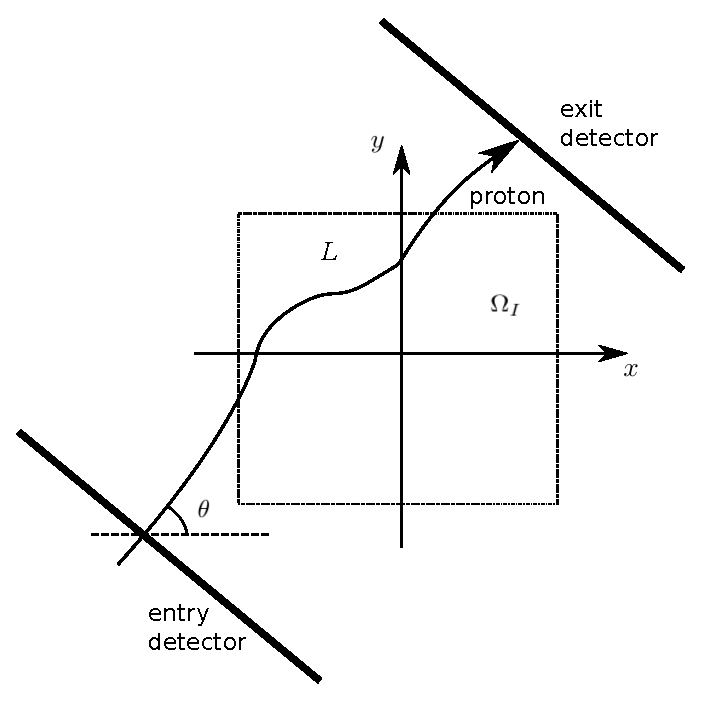
\includegraphics[scale=0.7]{img/param2.eps}
\caption{A proton travelling through the image reconstruction region (dashed square). The entry and exit detectors (solid lines) measure the position and direction of the proton before and after the phantom. The exit detector also measures the proton's residual energy. $L$ is the path the proton travels between the two detectors. The dashed square is the reconstruction region $\Omega_I$.}
\label{fig:param}
\end{figure}

Two phantoms were designed to investigate the spatial resolution and the relative stopping power accuracy of both imaging algorithms. The phantoms and simulation details are discussed in section \ref{sec:simulations}.

\subsection{Path estimates}
\label{sec:pathestimates}
Estimates of the proton paths through the reconstruction region can be calculated based on their position and direction measured by the CT detectors. The three most common path estimates used in the literature are the straight path, the cubic spline path and the most likely path (MLP). The straight path and cubic spline path estimates involve fitting the entry and exit position and direction at the phantom boundaries to a straight line or cubic function. The MLP estimate is the statistically most likely trajectory of a proton given the position and direction at the entry and exit detectors, and is based on the assumption that the angular scattering and lateral displacement of the proton obeys a Gaussian distribution \parencite{eyges1948multiple}. The reader is directed to \parencite{schulte2008maximum} and \parencite{williams2004most} for the mathematical formalism. A comparison of the path estimates has been performed and showed that the most likely path estimate predicts the path of the proton to the highest degree of accuracy, followed by the cubic spline and then the straight path \parencite{li2006reconstruction}. This work compares the use of the cubic spline path and the most likely path (MLP).


\subsection{Backprojection-then-filtering}
\label{sec:BPF}
The backprojection-then-filtering algorithm (BPF) for image reconstruction was first suggested by Bates and Peters \parencite{bates1971towards}, however the filtered backprojection method (FBP) is the favoured analytical approach in clinical use today. This is due to the large amounts of memory and longer computation times needed for BPF, as well as BPF suffering from quantitative inaccuracies. Studies comparing BPF and FBP have shown that, in general, BPF is inferior to FBP \parencite{suzuki1988comparison}. However, BPF naturally lends itself to the curved trajectories of protons. 

In recent work, the BPF algorithm was applied to simulated proton CT data, where the proton paths were fitted to a cubic spline \parencite{poludniowski2014proton}. In what follows, the BPF algorithm is presented as proposed by Poludniowski et al.

The BPF algorithm strongly resembles the filtered backprojection, but as the name suggests the ordering of the filtering and the backprojection is reversed. The algorithm consists of the following steps:
\begin{enumerate}
\item Backproject the (unfiltered) projection data, $g_k(\theta)$, from each view angle $\theta$ on to a 2D backprojection matrix, $b(x,y)$
\item Filter the backprojection matrix $b(x,y)$ using an appropriate filtering kernel
\end{enumerate}

\subsubsection{Backprojection}
The backprojection operation is equivalent to smearing the individual projections along the paths of the protons onto a backprojection matrix. In the case of the FBP algorithm, the backprojection step assumes straight paths for the imaging particles. By reversing the order of the backprojection and filtering operations, it is possible to backproject the projections along the curved path estimates (see section \ref{sec:pathestimates}).

For a computer implementation, the backprojection regions can be discretised onto a 2D backprojection matrix of voxels of pitch $\tau$, $b[i,j]$, where $i = 1 \dots M$ and $j = 1 \dots M$ and $x_{i} = (2i - M - 1)\tau/2$ and $y_j = (2j - M - 1)\tau/2$. If $L$ is the number of equally space projection angles about $\pi$ rad ($ l = 1 \dots L$, and projection angle $\theta = \pi (l - 1)/L$), the $M \times M$ backprojection matrix can then be expressed as

\begin{align}
\label{eq:bp}
%b[i,j] = \frac{\pi}{L}\sum_{l=1}^L \frac{\sum_{k=1}^K \lambda_{k,l}[i,j] g[k,l]}{\sum_{k=1}^{K} \lambda_{k,l}[i,j]}
b[i,j] & = \frac{\pi}{L}\sum_{l=1}^L b_l[i,j] \\
\text{where} \nonumber\\
b_l[i,j] & = \frac{\sum_{k=1}^K \lambda_{k,l}[i,j] g[k,l]}{\sum_{k=1}^{K} \lambda_{k,l}[i,j]} \label{eq:angularbpf}
\end{align}
where $k=1 \dots K$ labels the $k^{th}$ proton ray, $g[k,l]$ is the projection from the $k^{th}$ ray at the $l^{th}$ view angle and $\lambda_{k,l}[i,j]$ is the path length traversed by the $k^{th}$ ray at the $l^{th}$ view through the $[i,j]$ pixel. In the case when the rotation is about $2\pi$ rad, the backprojection matrix is half of that in equation \ref{eq:bp}.

The BPF algorithm is known to be more accurate with increasing size of backprojection matrix (see section \ref{sec:BPFfiltering}). As such, the backprojection matrix can be extrapolated by extrapolating the paths of the protons. Figure \ref{fig:backproject} shows a typical proton path along which a proton is backprojected.

\begin{figure}[!htb]
\centering
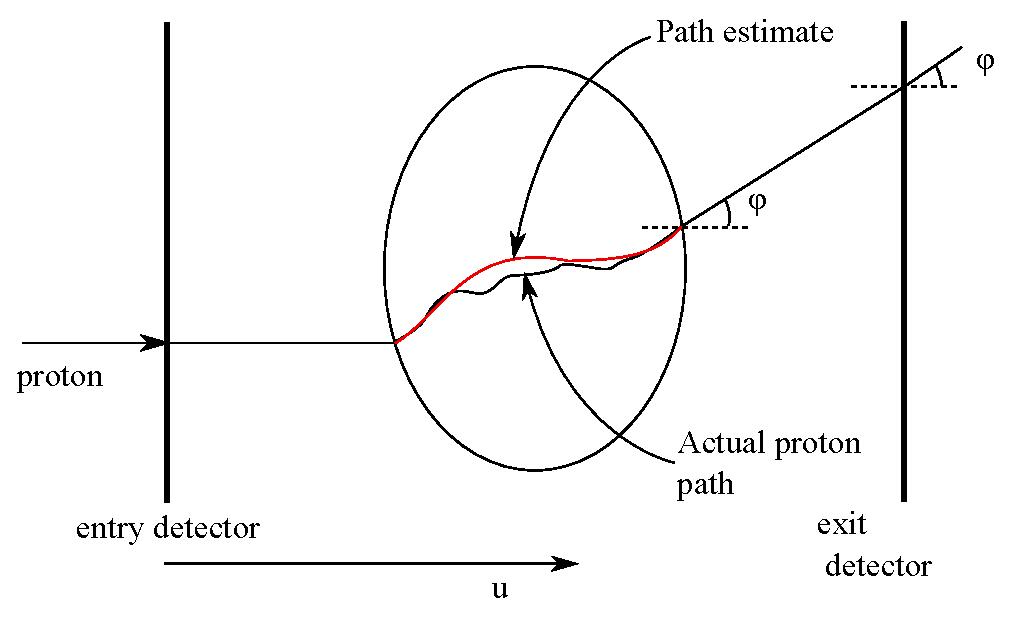
\includegraphics[scale=0.5]{img/backproject.eps}
\caption{(Exaggerated) path of a proton as it is deflected inside the elliptical phantom. The red line shows a path estimation for the proton based on position and direction measured by the entry and exit detectors.}
\label{fig:backproject}
\end{figure}
%Intersection indices and path lengths of the proton rays with the voxels in the voxel space can be determined using Siddon's algorithm.

%If the projections are about $2 \pi$ rad a factor of $1/2$ is introduced to equation \ref{eq:bp}.

\subsubsection{Filtering}
\label{sec:BPFfiltering}
%The approach to finding a filter resembles that used for the FBP. 
The backprojection function, $b(x,y)$, has been shown to be related to the original function being imaged, $f(x,y)$, by a 2D convolution (denoted **) \parencite{zeng1994backprojection},

\begin{eqnarray}
\label{eq:bpblur}
b(x,y) = f(x,y) ** \frac{1}{r}
\end{eqnarray}
where $r = |(x,y)|$. The original image can thus be obtained by a 2D convolution with a spatial kernel $k(x,y)$,
\begin{align}
f(x,y) & = \mathcal{F}^{-1}\left(\frac{\mathcal{F}(b)}{\mathcal{F}(r^{-1})}\right) \\
& = b(x,y) ** \mathcal{F}^{-1}(\omega) \nonumber\\
& = b(x,y) ** k(x,y) \nonumber
\end{align}
where $\omega = |(\omega_x,\omega_y)|$ and $(\omega_x,\omega_y)$ are the conjugate frequency variables to $(x,y)$. Due to the pitch $\tau$ of the backprojection matrix, in a computer implementation the backprojection region is sampled at a frequency $1/\tau$. Thus the Nyquist frequency must be imposed on the calculation of the spatial kernel, in a similar manner to the case of the FBP filter. The analytical form of $k(r)$ has been shown to be \parencite{poludniowski2014proton}
\begin{align}
k(r) & = \mathcal{F}^{-1}(\omega) \\
& = \frac{1}{4\pi^2r^3}\left[\left(\frac{\pi r}{\tau}\right)^2 J_1\left(\frac{\pi r}{\tau}\right) - \phi\left(\frac{\pi r}{\tau}\right)\right] \nonumber\\
\text{where} & \nonumber\\
\phi(x) & = \frac{\pi x}{2} [ J_1(x) H_0(x) - J_0(x) H_1(x)]\nonumber
\end{align}
where $J_n$ and $H_{n}$ are the $n^{th}$ order Bessel and Struve functions respectively. To avoid divergence and keep the kernel finite at $r = 0$, 
\begin{align}
k(r=0) = \frac{\pi}{12\tau^3}.
\end{align}
The imaged function in its discretised form is thus given by
\begin{eqnarray}
f[i,j] = b[i,j] ** k[i,j] 
\label{eq:bpconv}
\end{eqnarray}
where $f[i,j]$ is the discretised reconstruction matrix of size $N \times N$ and $i$ and $j$ are integer values, $i = 1 \dots N$  and $j = 1 \dots N$. The filtering is typically performed in the frequency domain and the spatial filtering kernel is fourier transformed, where appropriate zero padding can be used to minimise aliasing and \textit{dishing} artefacts.

The BPF algorithm is known to suffer from a constant offset in the reconstructed values \parencite{suzuki1988comparison}. Due to the nature of the convolution in equation \ref{eq:bpblur}, the backprojection $b(x,y)$ is non zero everywhere, even though outside the domain of the reconstruction region $f(x,y) = 0$. In a computer implementation of equation \ref{eq:bpconv}, the backprojection matrix must be truncated and leads to lower reconstructed values. A larger backprojection matrix leads to quantitatively more accurate results but the offset is still apparent. The addition of a correction term can be used to try to rectify this,

\begin{eqnarray}
\Delta = \left( \tau^2 \sum_{\substack{\text{pixels in}\\\text{reconstruction}\\\text{region}}} f[i,j] \right) \left( \tau^2 \sum_{\substack{\text{pixels not in}\\\text{reconstruction}\\\text{region}}} \frac{k[N/2 - i, N/2 - j]}{\tau\sqrt{i^2 + j^2}}\right)
\label{eq:correction}
\end{eqnarray}
that can be added to all reconstructed values for an improved quantitative accuracy,
\begin{eqnarray}
f_{\Delta}(x,y) = f(x,y) + \Delta
\end{eqnarray}

\subsection{Derivative Hilbert Backprojection}
\label{sec:HBP}
A two step Hilbert transform method was first proposed by Noo et al for 2D images obtained from a parallel beam geometry \parencite{noo2004two}. The advantage of this algorithm over the FBP algorithm is that it is able to reconstruct images from truncated projection data \parencite{defrise2006truncated}. Noo's two step Hilbert transform method consists of the following steps:
\begin{enumerate}
\item Bin the projection data at the detector according to location (as in FBP)
\item Find the first derivatives of the projection data with respect to neighbouring bins
\item Backproject the derivatives to form a backprojection matrix
\item Perform a finite inverse Hilbert transform of the backprojection matrix to retrieve the image, $f(x,y)$
\end{enumerate}
Zeng proposed the reversal of the order of the backprojection and differentiation operations for an algorithm more well suited for list mode data \parencite{zeng2007image}. In his method, the raw projection data is backprojected first and derivatives are taken second. This switch allows for the inclusion of the proton path estimates in to the two step Hilbert transform algorithm. Furthermore, the finite Hilbert transform does not demand an unbounded backprojection matrix and thus the error resulting from the backprojection matrix truncation in the BPF is eliminated.

\subsubsection{Backprojection}
\label{sec:bphbp}
The backprojection function is the sum of derivatives of two weighted backprojection functions. If the projections span $180^{\circ}$, the two weighted backprojection functions, $b_x(x,y)$ and $b_y(x,y)$, are given by
\begin{align}
b(x,y) & = \frac{\partial}{\partial x} b_{x}(x,y) + \frac{\partial}{\partial y} b_{y}(x,y) \\
\text{where} & \\
b_x(x,y) & = \int_{0}^{\pi} (-1) b_{\theta}(x,y) \sin \theta d \theta, \\ 
b_y(x,y) & = \int_{0}^{\pi} b_{\theta}(x,y) \cos \theta d\theta
\end{align}
where $b_{\theta}(x,y)$ is a backprojection from the projection angle $\theta$. If the projections span $360^{\circ}$, then
\begin{align}
b_x(x,y) & = \frac{1}{2} \int_{0}^{\pi} (-1) b_{\theta}(x,y) \sin \theta d \theta + \frac{1}{2} \int_{\pi}^{2\pi} b_{\theta}(x,y) \sin \theta d \theta,  \\ 
b_y(x,y) & = \frac{1}{2} \int_{0}^{\pi} b_{\theta}(x,y) \cos \theta d\theta + \frac{1}{2} \int_{\pi}^{2\pi} (-1) b_{\theta}(x,y) \cos \theta d\theta
\end{align}
On a computer, the angular backprojections $b_{\theta}(x,y)$ are replaced with their discretised versions as in section \ref{sec:BPF}, equation \ref{eq:angularbpf}.

The choice of the axis defining $\theta$ (see figure \ref{fig:backproject}) is irrelevant for the algorithm except when performing a reconstruction from truncated data. Such cases are not handled in this work, but further information can be found in Zeng and Noo's work.

\subsubsection{Finite inverse Hilbert transform}
\label{sec:invhil}
Each row of elements along the $x$ axis in the backprojection matrix from section \ref{sec:bphbp} is the Hilbert transform of the image function. Thus to obtain the image function, the inverse Hilbert transform of each row of $b(x,y)$ needs to be calculated. However, since $f(x,y) = 0$ outside the domain of the reconstruction region, the inverse operation reduces to the finite inverse Hilbert transform \parencite{zeng2007two},
%\begin{eqnarray}
%b(x,y) = 2 \pi  \textbf{H} [f(x,y)].
%\end{eqnarray}

\begin{eqnarray}
f(x,y) = \frac{1}{2\pi} \textbf{H$_{x}$}^{-1} b(x,y)
\end{eqnarray}
where \textbf{H$^{-1}_x$} is the inverse Hilbert transform along the $x$ axis. In this work, the finite inverse Hilbert formula shown in \parencite{zeng2007two}, equation (9), was used. % The ref is Two Finite Inverse Hilbert Transform Formulae for Region-of-Interest Tomography
%\begin{eqnarray}
%f(x,y) & = \frac{1}{\sqrt{R^2 - x^2} - \sqrt{r^2 - x^2}} \int_{-R}^{+R} \frac{k(R,r,s)}{x-s}b(s,y)ds \\
%\text{where}
%k(R,r,t) = \begin{cases}
%-\sqrt{R^2 - t^2}/\pi \\
%-\sqrt{R^2 - t^2}/\pi + \sqrt{r^2 - t^2}/\pi \\
%0
%\end{cases}
%\end{eqnarray}

\subsection{Simulations}
\label{sec:simulations}
All proton CT data was obtained via Monte Carlo simulations using the GEANT4 10.2.1 (GEometry ANd Tracking) simulation toolkit \parencite{agostinelli2003geant4}. Originally developed for high energy particle physics applications, GEANT4 is able to simulate particles propagating through and interacting with matter. The C++ based software has more recently found its place in medical applications. Using GEANT4, protons can be generated and tracked as they travel through a phantom and detectors can be designed to measure quantities such as energy, position and momentum. Furthermore, an abundance of physical processes are available to handle the diverse interactions that may occur over a wide energy range. In essence, it is possible to implement a virtual proton CT system and virtual phantoms. 

%Proton CT simulations in this work were performed used GEANT4 10.2.1 [ref] with
All proton CT data was obtained via Monte Carlo simulations using the GEANT4 10.2.1 (GEometry ANd Tracking) simulation toolkit \parencite{agostinelli2003geant4}. The physics list QGSP\_BERT was used to define the physical processes as it includes standard electromagnetic and hadronic processses. The backprojections were performed using C++, and the RSP reconstructions and analysis of the results were carried out in MATLAB 2014a. The Struve functions for the filtering step in the BPF algorithm were computed using the FORTRAN library routines by Zhang and Jin \parencite{zhang16computation} translated into MATLAB using f2matlab \parencite{f2matlab}.

Two phantoms were chosen to be imaged. The design of the first phantom was taken from \parencite{rit2015list}, which is referred to as the rod phantom, and consists of aluminium rods of 5 mm diameter (material: G4\_Al) positioned at increasing radial distances from the centre of a cylindrical volume of water (material: G4\_WATER) of 20 cm diameter in a spiral orientation. This was used in an effort to mimic the spatial resolution results obtained by Rit \parencite{rit2015list}. The second phantom imaged was a Shepp Logan head phantom used to assess RSP accuracy \parencite{shepp1974fourier} with semi major and semi minor axis of 119.7 mm and 89.7 mm respectively. The head phantom consisted of air (G4\_AIR), water (G4\_WATER), bone (G4\_BONE\_COMPACT\_ICRU) and brain (G4\_BRAIN\_ICRP) materials. Both phantoms had a height of 10 cm. They are shown in figure \ref{fig:phantom}.

\begin{figure}[htp]
  % Fixed length
  \centering
  \subcaptionbox{\label{fig3:a}}{\includegraphics[width=0.325\linewidth]{img/phantomsetup.png}}\hspace{0.5em}%
  \subcaptionbox{\label{fig3:b}}{\includegraphics[width=0.3\linewidth]{img/rodphantom.png}}\hspace{0.5em}%
 \subcaptionbox{\label{fig3:c}}{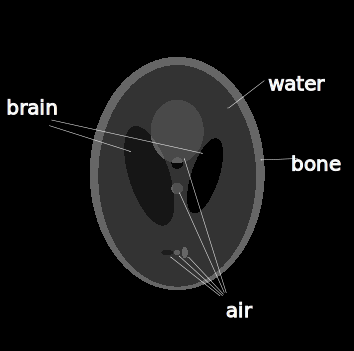
\includegraphics[width=0.27\linewidth]{img/shepploganphantom.png}}
 \caption{GEANT4 images: Figure \ref{fig3:a} - rod phantom positioned at the centre of two square detectors. Figure \ref{fig3:b} - rod phantom made up a cylindrical volume of water with 23 aluminium rods of 5 mm diameter distributed in a spiral. Figure \ref{fig3:c} - Shepp Logan head phantom consisting of water, air, bone and brain.}
\label{fig:phantom}
\end{figure}

Entry and exit detectors were positioned 23 cm away from the phantom centre. Each detector was 30 x 30 cm$^2$ and measured the position and direction of individual protons as they passed through. The exit detector also measured the individual protons' kinetic energy. A uniformly distributed 200 MeV proton beam with no energy distribution and divergence was used. This energy was chosen to ensure that the majority of protons passed through the entire phantom and arrived at the exit detector as well as being an attainable energy in a clinical setting. The beam spanned a 26 cm line parallel to the detector, with the proton beam direction perpendicular to the detector and directed towards the phantom. In the case of imaging the rod phantom, $4 \times 10^5$ protons were used every $0.5^{\circ}$. For imaging of the head phantom, $10^5$ protons were generated every $1^{\circ}$. In both cases, the proton beam rotated $360^{\circ}$ about the phantom. $3\sigma$ cuts on relative exit angle and on absolute lateral displacement between entry and exit detectors were imposed on the data to filter out protons that had likely undergone an inelastic interaction. For the case of the Shepp-Logan phantom, 87.2\% of the fired protons were detected at the exit detector, and of those 97.6\% were kept after applying cuts $3\sigma$ cuts. In the case of the rod phantom, 90.6\% of the fired protons arrived at the exit detector and 97.7\% of those remained after applying cuts. No filtering was applied to the images after reconstruction.


\subsection{Spatial resolution and RSP accuracy}
To assess the quality of the images obtained using either algorithm, the spatial resolution and the quantitative accuracy of the RSPs need to be taken into consideration. There are various methods of measuring spatial resolution. In this work the method proposed by Rit was used \parencite{rit2015list}.

The algorithms' spatial resolution capability was assessed using the rod phantom. Rit's method involves sampling line profiles along radial lines from the centre of each rod to a distance of 4 mm. 360 radial profiles were sampled at $1^{\circ}$ integrals, and the average normalised radial profile was fitted to a gaussian error function. The standard deviation, $\sigma$, was chosen as a measure of the spatial resolution. 

To assess RSP accuracy, three regions of interest (ROI) were selected within the Shepp Logan phantom. The three ROI consisted of either water, air or brain with RSPs of 1.0, 0.0011, 1.0428. The materials used came from the NIST reference database \parencite{nist} and the RSPs were obtained directly from GEANT4 after modification of the TestEm0 example application package with the toolkit. The mean RSP and standard deviation were calculated within each ROI to assess image accuracy and noise respectively. 


\section{Results}
%\begin{figure}[!htb]
%\centering
%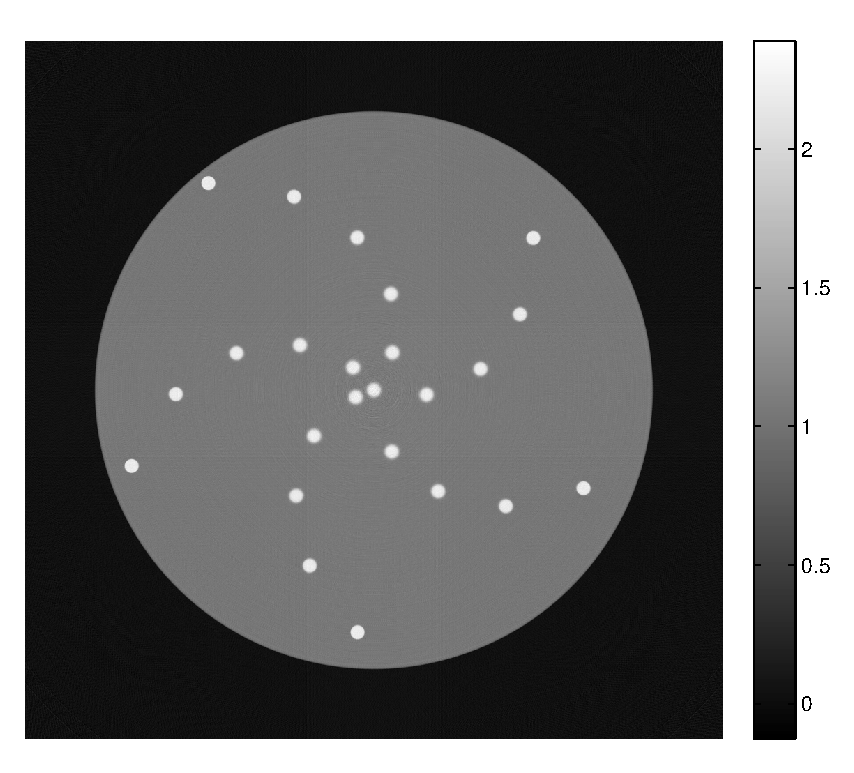
\includegraphics[scale=0.5]{img/BPFMLPimg.eps}
%\end{figure}



\subsection{Most likely path in water}
The MLP calculation was implemented using the method described by \cite{schulte2008maximum}. Protons were simulated to travel through 20 cm of water using GEANT4, and their speed and momentum was measured every 0.5 cm. The function $1/(\beta^2p^2)$ was then fitted to a $5^{th}$ degree polynomial, $\sum_{i=0}^{5} a_{i} u^{i}$, where $u$ is the penetration depth of the proton, $\beta$ is the speed of the proton relative to the speed of light, $p$ is the momentum of the proton, and $a_i$ are the polynomial coefficients. The polynomial coefficients are shown in table \ref{fig:coefficients}.

\begin{table}[h]
\centering
\caption{Polynomial coefficients used to fit the curve $1/(\beta^2 p^2) = \sum_{i=0}^5 a_i u^i$. The coefficients $a_{i}$ are in units of c$^2$/MeV divided by appropriate powers of cm. Strict cuts of $3\sigma$ were applied on proton kinetic energy and on exit angle relative to entry angle before fitting.}
\begin{tabular}{l|c}
\hline
Coefficient & $a_{i}$ (c$^2$/(MeV cm$^{i})$) \\ \hline
$a_0$ & $7.4361\times 10^{-6}$ \\
$a_1$ & $5.0199\times 10^{-7}$ \\
$a_2$ & $-7.8071 \times 10^{-8}$ \\ 
$a_3$ & $1.5860 \times 10^{-8}$ \\
$a_4$ & $-1.0912 \times 10^{-9}$ \\
$a_5$ & $3.0185 \times 10^{-11}$  \\
\end{tabular} 
\label{fig:coefficients}
\end{table}

\subsection{Reconstruction}

The BPF and HBP algorithm were used to reconstruct RSPs of the rod phantom and the Shepp Logan phantom. Reconstructed images of the BPF algorithm are shown in figure \ref{fig:reconstruction} (HBP reconstruction images omitted here). 

The reconstruction voxels were chosen to be 0.25 mm $\times $ 0.25 mm and 1 mm $\times$ 1 mm when imaging the rod phantom and Shepp Logan phantom respectively. In both cases, the reconstruction region was centred at the isocentre. In the case of HBP, the backprojection matrix was a 25 cm $\times$ 25 cm square, while for the BPF algorithm a larger backprojection matrix of dimensions 100 cm $\times$ 100 cm was used to minimise truncation errors, created by extrapolating the proton paths beyond the detectors. The cubic spline and most likely paths were constructed as piece wise linear, where each piece is approximately 1 mm. The mean ionisation potential for water used in the numerical integration of equation \ref{eq:WEPL} was $I_{water} = 78$ eV as per GEANT4.

\subsubsection{Spatial resolution}
\label{sec:spatialresolution}
A plot of $\sigma$ as a function of distance from the centre of the rod phantom is shown in figure \ref{fig:resolution}. The lowest spatial resolution was observed at the centre of the phantom, and increased with radial distance from the centre. This is to be expected as the cubic spline and most likely path estimates are most accurate close to the edges of the phantom. A significant improvement in spatial resolution can be observed when using the MLP over the cubic spline path, both for the BPF and HBP algorithms. At the edge of the phantom, this difference in resolution diminishes due to the accuracy of the MLP and cubic spline being almost equal.

A small improvement in spatial resolution can be observed when comparing the BPF and HBP reconstructions when using both path estimates. Defining $\Delta \sigma = \sigma_{BPF} - \sigma_{HBP}$, then when using the cubic path estimates $|\Delta \sigma|_{max} =3.07 \times 10^{-4}$ and $|\Delta \sigma|_{min} = 0.0249$, and when using the MLP $|\Delta \sigma|_{max} = 0.0227$, $|\Delta \sigma|_{min} = 0.0054$. Once again, the improvement diminishes towards the edge of the phantom.


\begin{figure}[!htb]
  \hspace*{\fill}%
  \subcaptionbox{\label{fig:rodPhantom}Rod phantom}{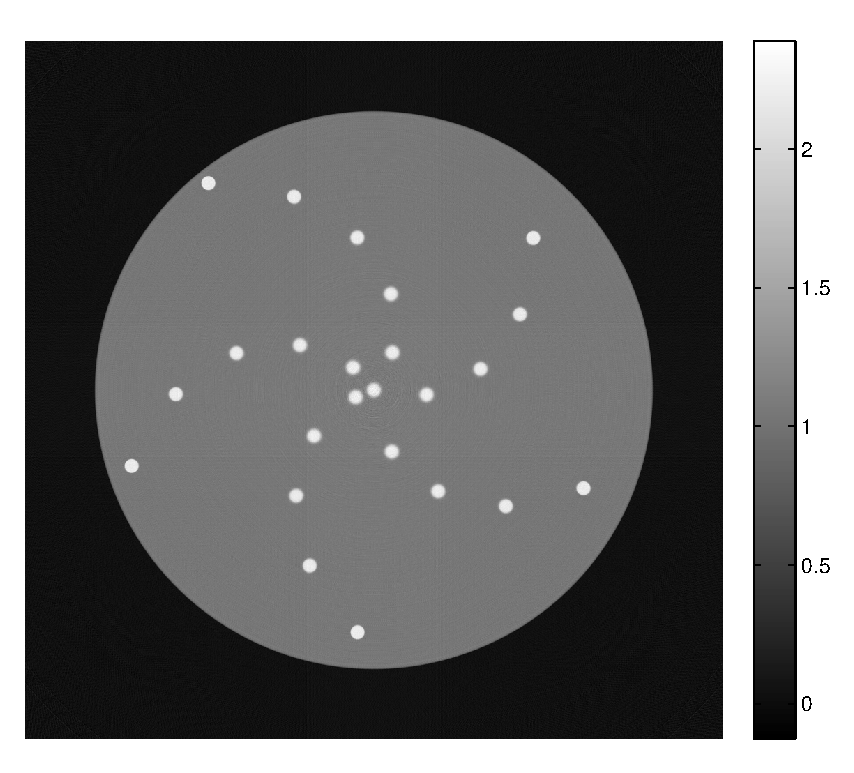
\includegraphics[width=2.4in]{img/BPFMLPimg.eps}}\hfill%
  \subcaptionbox{  \label{fig:sheppphantom}Shepp Logan phantom}{\includegraphics[width=2.4in]{img/BPFSheppMLPimg.eps}}%
  \hspace*{\fill}\\
  \caption{RSP reconstructions for the rod phantom (figure \ref{fig:rodPhantom}: $1000 \times 1000$ pixels, 1 pixel = $0.25 \times 0.25$ mm$^2$) and the Shepp Logan phantom (figure \ref{fig:sheppphantom}: $250 \times 250$ pixels, 1 pixel = $1 \times 1$ mm$^2$). Both images reconstructed using the BPF algorithm. Similar results can be seen for the HBP algorithm, not shown here.}
  \label{fig:reconstruction}
\end{figure}


\begin{figure}[!htb]
\centering
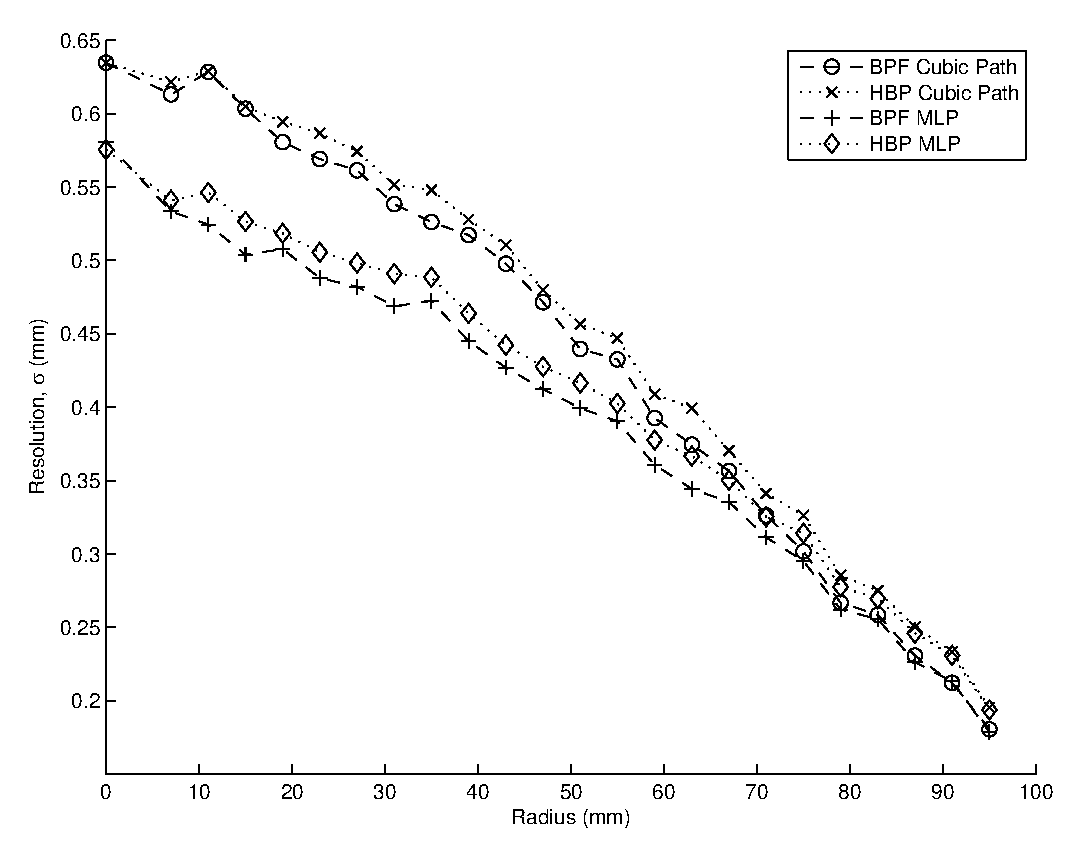
\includegraphics[scale=0.6]{img/resolution.eps}
\caption{Plot of spatial resolution using BPF and HBP algorithm with cubic path and most likely path estimates, determined from reconstructed images of rod phantom. Spatial resolution $\sigma$ as defined in section \ref{sec:spatialresolution} was used.}
\label{fig:resolution}
\end{figure}

\subsubsection{RSP accuracy}

The mean relative stopping powers (RSP) and standard deviations of three regions of interest (ROI) within the Shepp Logan head phantom are shown in table \ref{table:RSPresultsBPF} (BPF) and table \ref{table:RSPresultsHBP} (HBP). For both algorithms, the mean RSP calculated for the ROI containing water was most accurate, while that containing air was least accurate. Comparisons of the RSP from both algorithms shows that the BPF algorithm produced slightly more accurate RSPs, but with a higher standard deviation. Using the most likely path resulted in an improvement in accuracy when compared to the cubic spline path estimate, as well as giving a lower standard deviation (Change in RSP between path estimates, $\Delta RSP \approx 10^{-4} \text{ to } 10^{-5}$).

%\begin{tabular}{l|cccc}
%\hline
%Material & RSP & Standard deviation, $\sigma$ & Percentage error\\ \hline
%Air (BPF (C))     & -0.006791 (-0.013485) & 0.008163 () & 133 \% \\
%Air (HBP (C))     & -0.009791 & 0.005126 &  990 \%\\
%Air (BPF (MLP))   & -0.006671 (-0.013365) & 0.008366 (0.008366) & 1320 \% \\
%Air (HBP (MLP))   & -0.009636 & 0.005120 & 976 \% \\
%Water (BPF (C))   & 1.010414 (1.003720) & 0.008778 () &  0.372 \% \\
%Water (HBP (C))   & 1.007362 & 0.005759 & 0.736 \% \\
%Water (BPF (MLP)) & 1.010367 (1.003673) & 0.008461 & 0.367 \% \\
%Water (HBP (MLP)) & 1.007315 & 0.005626 & 0.732 \% \\
%Brain (BPF (C))   & 1.062785 (1.056091) & 0.010883 () & 1.27 \% \\
%Brain (HBP (C))   & 1.056655 & 0.007720 & 1.33 \% \\
%Brain (BPF (MLP)) & 1.062725 (1.056030) & 0.010683 & 1.27 \%\\
%Brain (HBP (MLP)) & 1.056479 & 0.007442 & 1.31 \% \\
%% things in brackets after correction...
%\label{table:RSPresults}
%\end{tabular} 

\begin{table}
\centering
\caption{Relative stopping powers reconstructed using the BPF algorithm with cubic spline path and most likely path estimates.}
\begin{tabular}{l|ccccc}
\hline
Material &  \multicolumn{2}{c}{RSP} & Standard deviation, $\sigma$ & Percentage error\\ \hline
Air (Cubic Path)     & -0.006791 & (-0.013485) & 0.008163  & 1330 \% \\
Air (MLP)   & -0.006671 & (-0.013365) & 0.008366 & 1320 \% \\
Water (Cubic Path)   & 1.010414 & (1.003720) & 0.008778 &  0.372 \% \\
Water (MLP) & 1.010367 & (1.003673) & 0.008461 & 0.367 \% \\
Brain (Cubic Path)   & 1.062785 & (1.056091) & 0.010883 & 1.27 \% \\
Brain (MLP) & 1.062725 & (1.056030) & 0.010683 & 1.27 \%\\
% things in brackets after correction...
\end{tabular} 
\label{table:RSPresultsBPF}
\end{table}

\begin{table}
\centering
\caption{Relative stopping powers reconstructed using the HBP algorithm with cubic spline path and most likely path estimates.}
\begin{tabular}{l|cccc}
\hline
Material & RSP & Standard deviation, $\sigma$ & Percentage error\\ \hline
Air (Cubic Path)     & -0.009791 & 0.005126 &  990 \%\\
Air (MLP)   & -0.009636 & 0.005120 & 976 \% \\
Water (Cubic Path)   & 1.007362 & 0.005759 & 0.736 \% \\
Water (MLP) & 1.007315 & 0.005626 & 0.732 \% \\
Brain (Cubic Path)   & 1.056655 & 0.007720 & 1.33 \% \\
Brain (MLP) & 1.056479 & 0.007442 & 1.31 \% \\
% things in brackets after correction...
\end{tabular} 
\label{table:RSPresultsHBP}
\end{table}
\section{Discussion}

The RSP reconstructions from the BPF algorithm exhibited an improvement in spatial resolution over the HBP algorithm. The path estimates were identical and hence backprojection operations from each projection angle were the same. The two significant differences between the backprojection matrices were that the BPF backprojection matrix was four times larger than the HBP backprojection matrix through extrapolation and that the HBP backprojection matrix is formed through the summation of two weighted backprojections. As expected, the spatial resolution of the images produced by both algorithms was highest when using the most likely path estimates, presumably because it more closely resembles the actual proton paths than the cubic path estimate.

With the exception of air, both the BPF and HBP algorithm overestimated the RSP of the selected ROIs in the head phantom. In the case of the BPF algorithm, this may in part be as a result of the truncation problem discussed in section \ref{sec:BPFfiltering}. Though a correction term was added to all reconstructed values, this may not completely alleviate the problem. Furthermore, in both algorithms it was assumed that the protons do not lose energy outside the phantom (i.e. in the surrounding air environment). In the case of imaging the head phantom, the proton travelled approximately 22 - 28 cm (depending on orientation of the phantom). The associated energy loss was not accounted for in the calculation of the WEPL which should lead to a small overestimation of RSP in the phantom.

Both the BPF and HBP algorithm underestimated the RSP of air using both path estimates, and reconstructed mean negative values in the chosen ROI. It is possible that the overestimation of the water and brain RSPs is linked to the underestimation of air RSP. This is a subject for further study.

By and large the most time consuming step of both algorithms was the backprojection operation. Siddon's algorithm was used to determine which voxels were intersected and the path length traversed by individual protons through each voxel \parencite{siddon1985fast}. The large $100 \times 100$ cm$^2$ backprojection matrix of $0.25 \times 0.25$ mm$^2$ voxels created by backprojecting approximately 280 million protons took approximately 9 hours, while backprojection of 36 million protons on to the $100 \times 100$ cm$^2$ backprojection matrix of $1 \times 1$ mm$^2$ voxels took approximately 40 minutes to create. The backprojections were performed using the high throughput computing cluster, condor [ref], at the University of Manchester. Because the backprojection operations are highly parallelisable, it is expected that similar or faster times should be obtainable using GPUs that can handle thousands of threads concurrently. The filtering stage for both algorithms is of the order of seconds.

The proton CT data that was simulated using GEANT4 involved an idealised set up with perfect tracking detectors to measure the position and direction of individual protons, from which the proton paths were estimated. The proton beam also had no spread of energies and the beam line was ideal. In a real system, the tracking detectors and calorimeter will have a limiting resolution and the beam will produce protons with a range of energies. In future work, a more realistic set up can be implemented in GEANT4 by account for these details, as well as using a customised physics list rather than the standard one, QGSP\_BERT, packaged with the toolkit. 

\section{Conclusion}
%Present treatment planning using x-ray CT can lead to errors in proton range of the order of 1-3 mm. Proton CT has the potential to measure directly the proton stopping powers relative to water and alleviating the necessity of 
The BPF and HBP reconstruction algorithms have been applied to simulated proton CT data to create maps of RSP. Two phantoms were imaged to assess and compare the capability of both algorithms: the rod phantom was used to assess the spatial resolution capabilities, while the Shepp Logan head phantom was used to assess the RSP accuracy. The cubic spline path and most likely path estimates were used as estimates of the proton track within the phantoms.

It was observed that when using the BPF or HBP algorithm, the most likely path estimates gave the highest spatial resolution when compared to the cubic path estimate. Regardless of which path estimate was chosen, the BPF algorithm produced images with a small improvement in resolution when compared to the HBP algorithm. 

The lowest percentage errors in mean RSP for water and brain were obtained using the most likely path estimate with the BPF algorithm. The RSP of the ROI containing air was underestimated and the reconstructions produced a negative mean RSP for air.

\section{Acknowledgements}
I would like thank Nick Henthorn, John Warmenhoven and Marios Satiropoulos for their support and useful advice regarding GEANT4.

%\bibliographystyle{ieeetr}
%\bibliography{bibfile}{}

%\bibliographystyle{unsrtnat}
\printbibliography

\end{document}

%\end{document}